%Iniziato a disegnare il grafo MST, ma mi sono rotto le balls a metà,
%Quindi vabbè un pezzo di grafo è qua, quando avrò sbatta lo completerò
% e sostituirò alle immagini
\begin{center}
    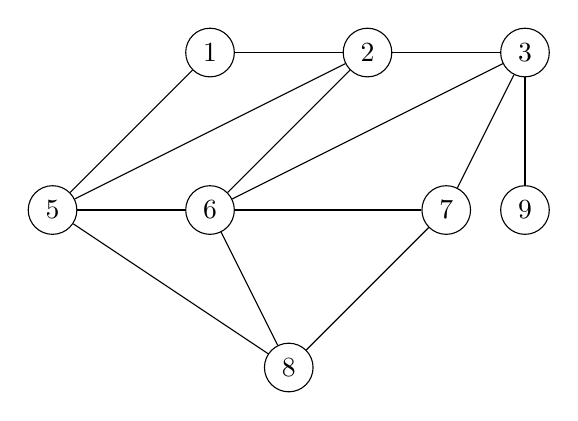
\begin{tikzpicture}
        \node[shape=circle,draw=black] (1) at (2,0) {1};
        \node[shape=circle,draw=black] (2) at (4,0) {2};
        \node[shape=circle,draw=black] (3) at (6,0) {3};
        %\node[shape=circle,draw=black] (4) at (6,0) {4};
        \node[shape=circle,draw=black] (5) at (0,-2) {5};
        \node[shape=circle,draw=black] (6) at (2,-2) {6};
        \node[shape=circle,draw=black] (7) at (5,-2) {7};
        \node[shape=circle,draw=black] (8) at (3,-4) {8};
        \node[shape=circle,draw=black] (9) at (6,-2) {9};
    
        \path [-] (1) edge (2);
        \path [-] (2) edge (3);
        %\path [-] (3) edge (4);
        \path [-] (1) edge (5);
        \path [-] (2) edge (5);
        \path [-] (2) edge (6);
        \path [-] (3) edge (6);
        \path [-] (3) edge (7);
        %\path [-] (4) edge (7);
        \path [-] (5) edge (6);
        \path [-] (6) edge (7);
        \path [-] (5) edge (8);
        \path [-] (6) edge (8);
        \path [-] (7) edge (8);
        \path [-] (3) edge (9);
    \end{tikzpicture}
    \end{center}